\documentclass[../AnalysisNoteJBuxton.tex]{subfiles}
\begin{document}

\subsection{Results: \texorpdfstring{$\Lambda$K$^{0}_{S}$ and $\Lambda$K$^{\pm}$}{TEXT}}
\label{ResultsLamK}

Figures \ref{fig:LamK0wConjFits}, \ref{fig:LamKchPwConjFits}, and \ref{fig:LamKchMwConjFits} (Section \ref{ResultsAndDiscussion}) show experimental data with fits for all studied centralities for $\Lambda$K$^{0}_{S}$ with $\bar{\Lambda}$K$^{0}_{S}$, $\Lambda$K$^{+}$ with $\bar{\Lambda}$K$^{-}$, and $\Lambda$K$^{-}$ with $\bar{\Lambda}$K$^{+}$, respectively.
The parameter sets extracted from the fits can be found in Tables \ref{tab:FitResultsLamK0} and \ref{tab:FitResultsLamKch}.
All correlation functions were normalized in the range 0.32 $< k^{*} <$ 0.40 GeV/c, and fit in the range 0.0 $< k^{*} <$ 0.30 GeV/c.
For the $\Lambda$K$^{-}$ and $\bar{\Lambda}$K$^{+}$ analyses, the region 0.19 $< k^{*} <$ 0.23 GeV/c was excluded from the fit to exclude the bump caused by the $\Omega^{-}$ resonance.
The non-flat background was fit with a linear form from 0.6 $< k^{*} <$ 0.9 GeV/c.
The theoretical fit function was then multiplied by this background during the fitting process.

In the figures (\ref{fig:LamK0wConjFits}, \ref{fig:LamKchPwConjFits}, and \ref{fig:LamKchMwConjFits}), the black solid line represents the ``raw" fit, i.e. not corrected for momentum resolution effects nor non-flat background.
The green line shows the fit to the non-flat background.  The purple points show the fit after momentum resolution and non-flat background corrections have been applied.
The initial values of the parameters is listed, as well as the final fit values with uncertainties.

For the $\Lambda$K$^{0}_{S}$ fits, $R$ was restricted to [2.0, 10.0 fm] and $\Lambda$ was restricted to [0.1, 0.8].
This gave the lowest $\chi^{2}$ value, but loosening this restriction changes the fit parameters slightly.
Notice, the 10-30\% radius is at its limit, as is $\lambda$ from the 30-50\% $\Lambda$K$^{0}_{S}$ analysis.
This accounts for the 0.000 systematic uncertainty of the 10-30\% $R$ value currently quoted in Table \ref{tab:FitResultsLamK0}.
An estimate for this uncertainty should be included in the next version of this note.
In the future, we may need to throw out the 30-50\% data from the fit, but this is not ideal.


\begin{figure}[h]
  \centering
  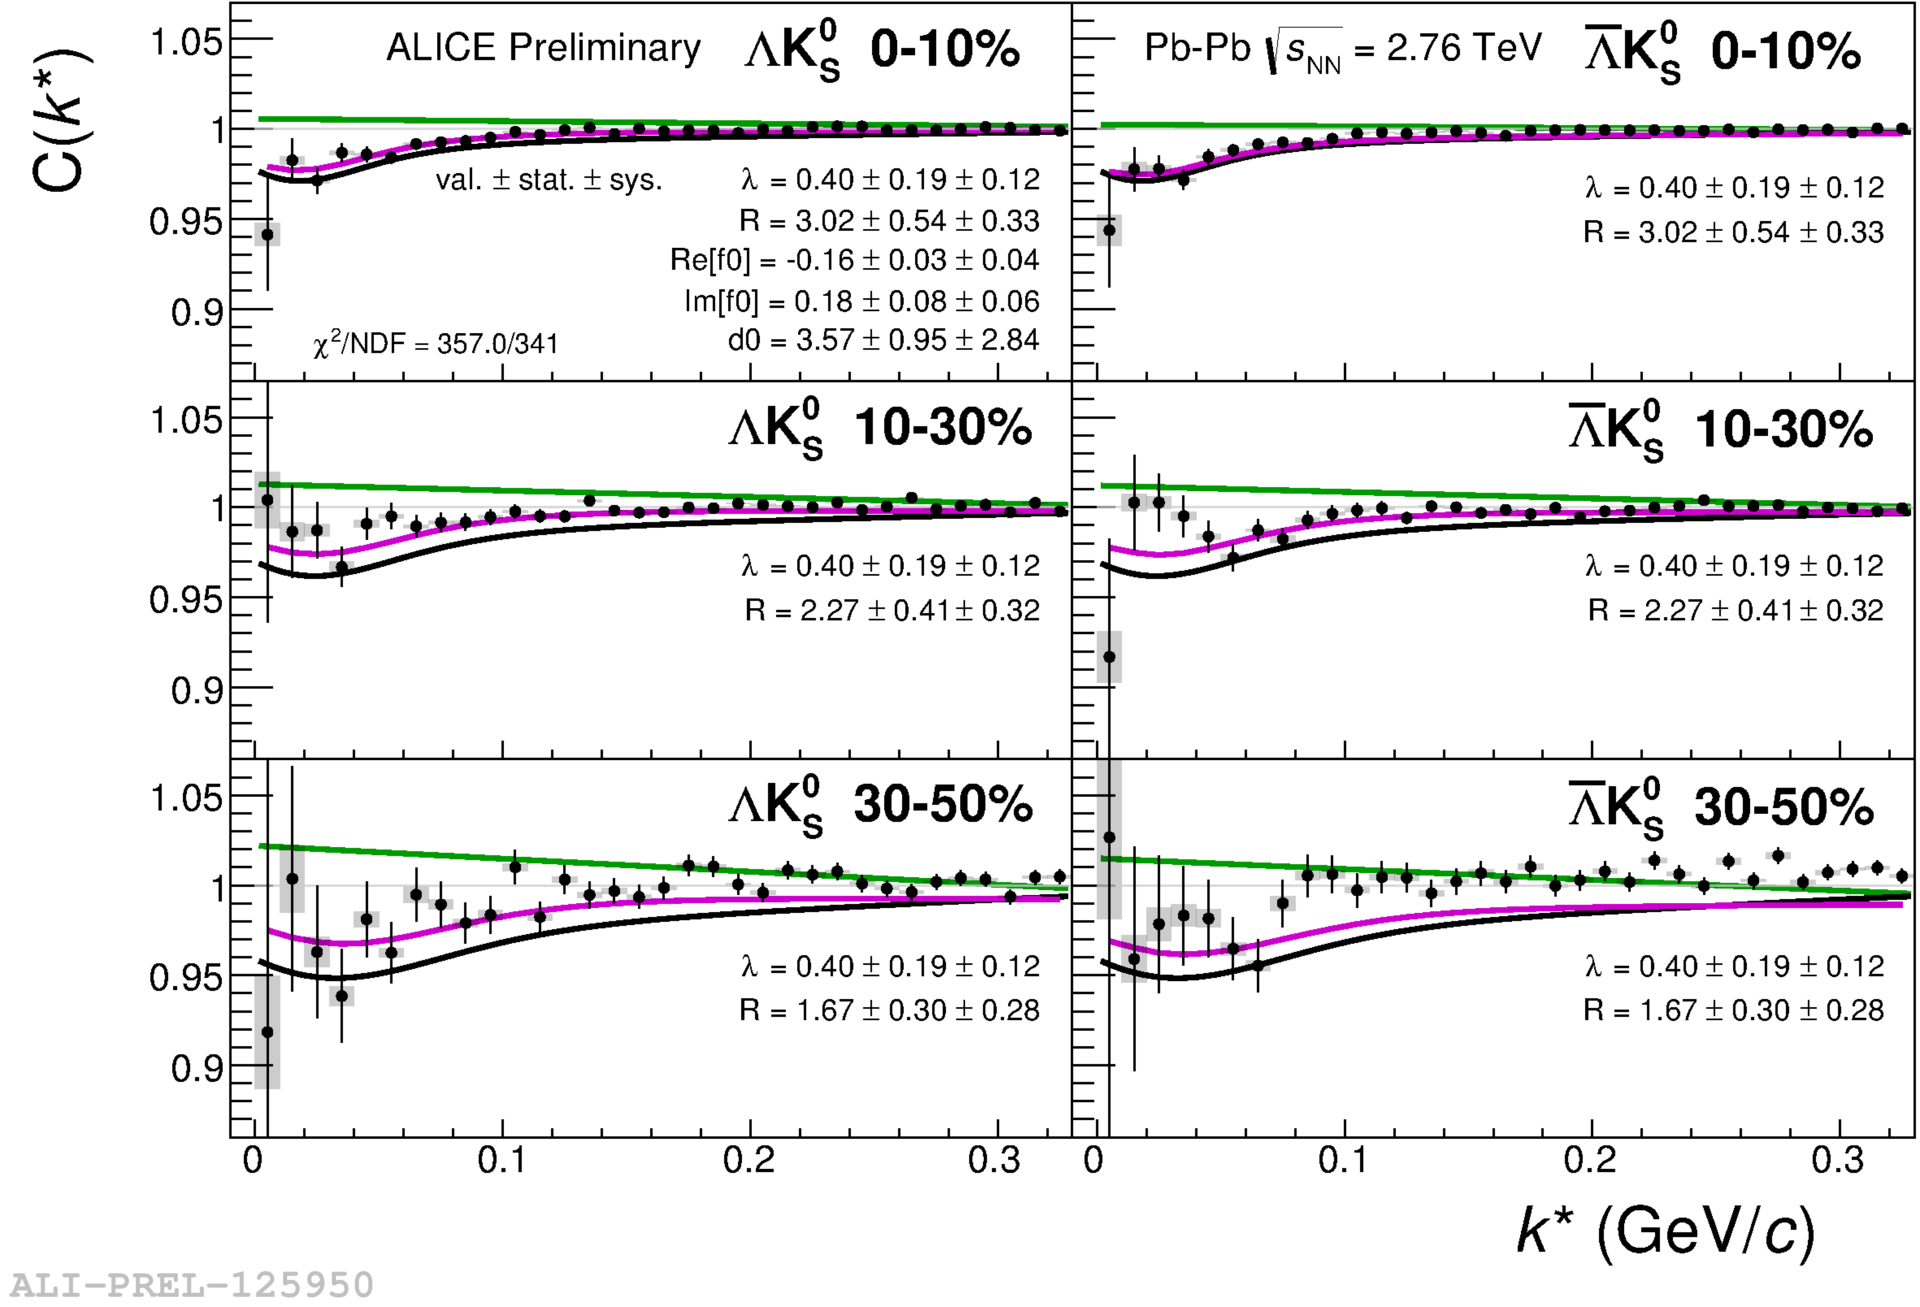
\includegraphics[width=\textwidth]{7_ResultsAndDiscussion/Figures/2017-Feb-03-canKStarCfwFitsLamK0wConj_0010_1030_3050_MomResCrctn_NonFlatBgdCrctn_SingleLamParam.png}
  \caption[$\Lambda$K$^{0}_{S}$($\bar{\Lambda}$K$^{0}_{S}$) Fits]{Fits to the $\Lambda$K$^{0}_{S}$ (left) and $\bar{\Lambda}$K$^{0}_{S}$ (right) data for the centralities 0-10\% (top), 10-30\% (middle), and 30-50\% (bottom).
The lines represent the statistical errors, while the boxes represent the systematic errors.
Each has unique $\lambda$ and normalization parameters.
The radii are shared amongst like centralities; the scattering parameters ($\mathbb{R}f_{0}$, $\mathbb{I}f_{0}$, $d_{0}$) are shared amongst all.
The black solid line represents the ``raw" fit, i.e. not corrected for momentum resolution effects nor non-flat background.  
The green line shows the fit to the non-flat background.
The purple points show the fit after momentum resolution and non-flat background corrections have been applied.
The initial values of the parameters is listed, as well as the final fit values with uncertainties.
Here, $R$ was restricted to [2.,10.] and $\Lambda$ was restricted to [0.1,0.8].}
  \label{fig:LamK0wConjFits}
\end{figure}

\begin{figure}[h]
  \centering
  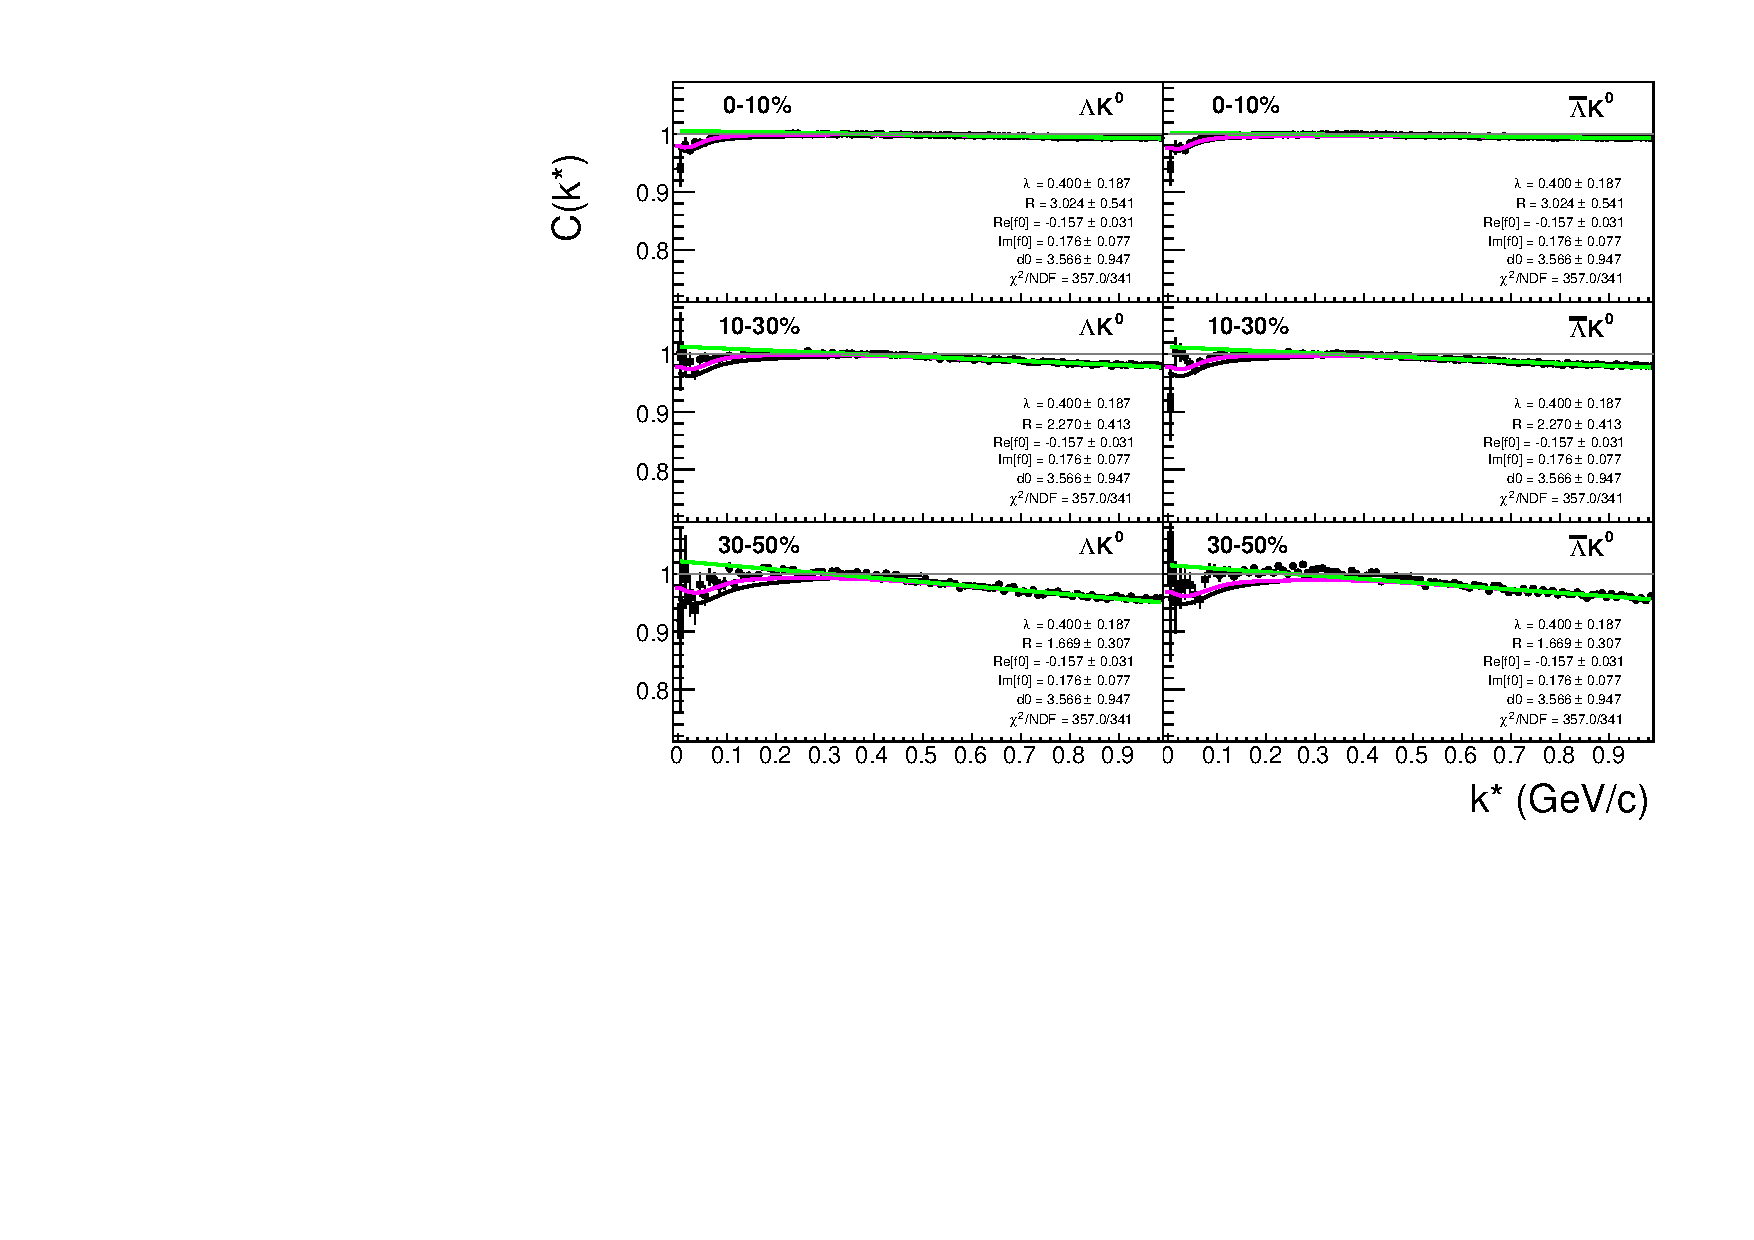
\includegraphics[width=\textwidth]{7_ResultsAndDiscussion/Figures/canKStarCfwFitsLamK0wConj_0010_1030_3050UnZoomed_MomResCrctn_NonFlatBgdCrctn.pdf}
  \caption[$\Lambda$K$^{0}_{S}$($\bar{\Lambda}$K$^{0}_{S}$) Fits (Wide Range)]{Same as Fig. \ref{fig:LamK0wConjFits}, but with a wider range of view.  
Fits to the $\Lambda$K$^{0}_{S}$ (left) and $\bar{\Lambda}$K$^{0}_{S}$ (right) data for the centralities 0-10\% (top), 10-30\% (middle), and 30-50\% (bottom).
The lines represent the statistical errors, while the boxes represent the systematic errors.
Each has unique $\lambda$ and normalization parameters.
The radii are shared amongst like centralities; the scattering parameters ($\mathbb{R}f_{0}$, $\mathbb{I}f_{0}$, $d_{0}$) are shared amongst all.
The black solid line represents the ``raw" fit, i.e. not corrected for momentum resolution effects nor non-flat background.  
The green line shows the fit to the non-flat background.
The purple points show the fit after momentum resolution and non-flat background corrections have been applied.
The initial values of the parameters is listed, as well as the final fit values with uncertainties.
Here, $R$ was restricted to [2.,10.] and $\Lambda$ was restricted to [0.1,0.8].}
  \label{fig:LamK0wConjFitsUnZoomed}
\end{figure}




\begin{figure}[h]
  \centering
  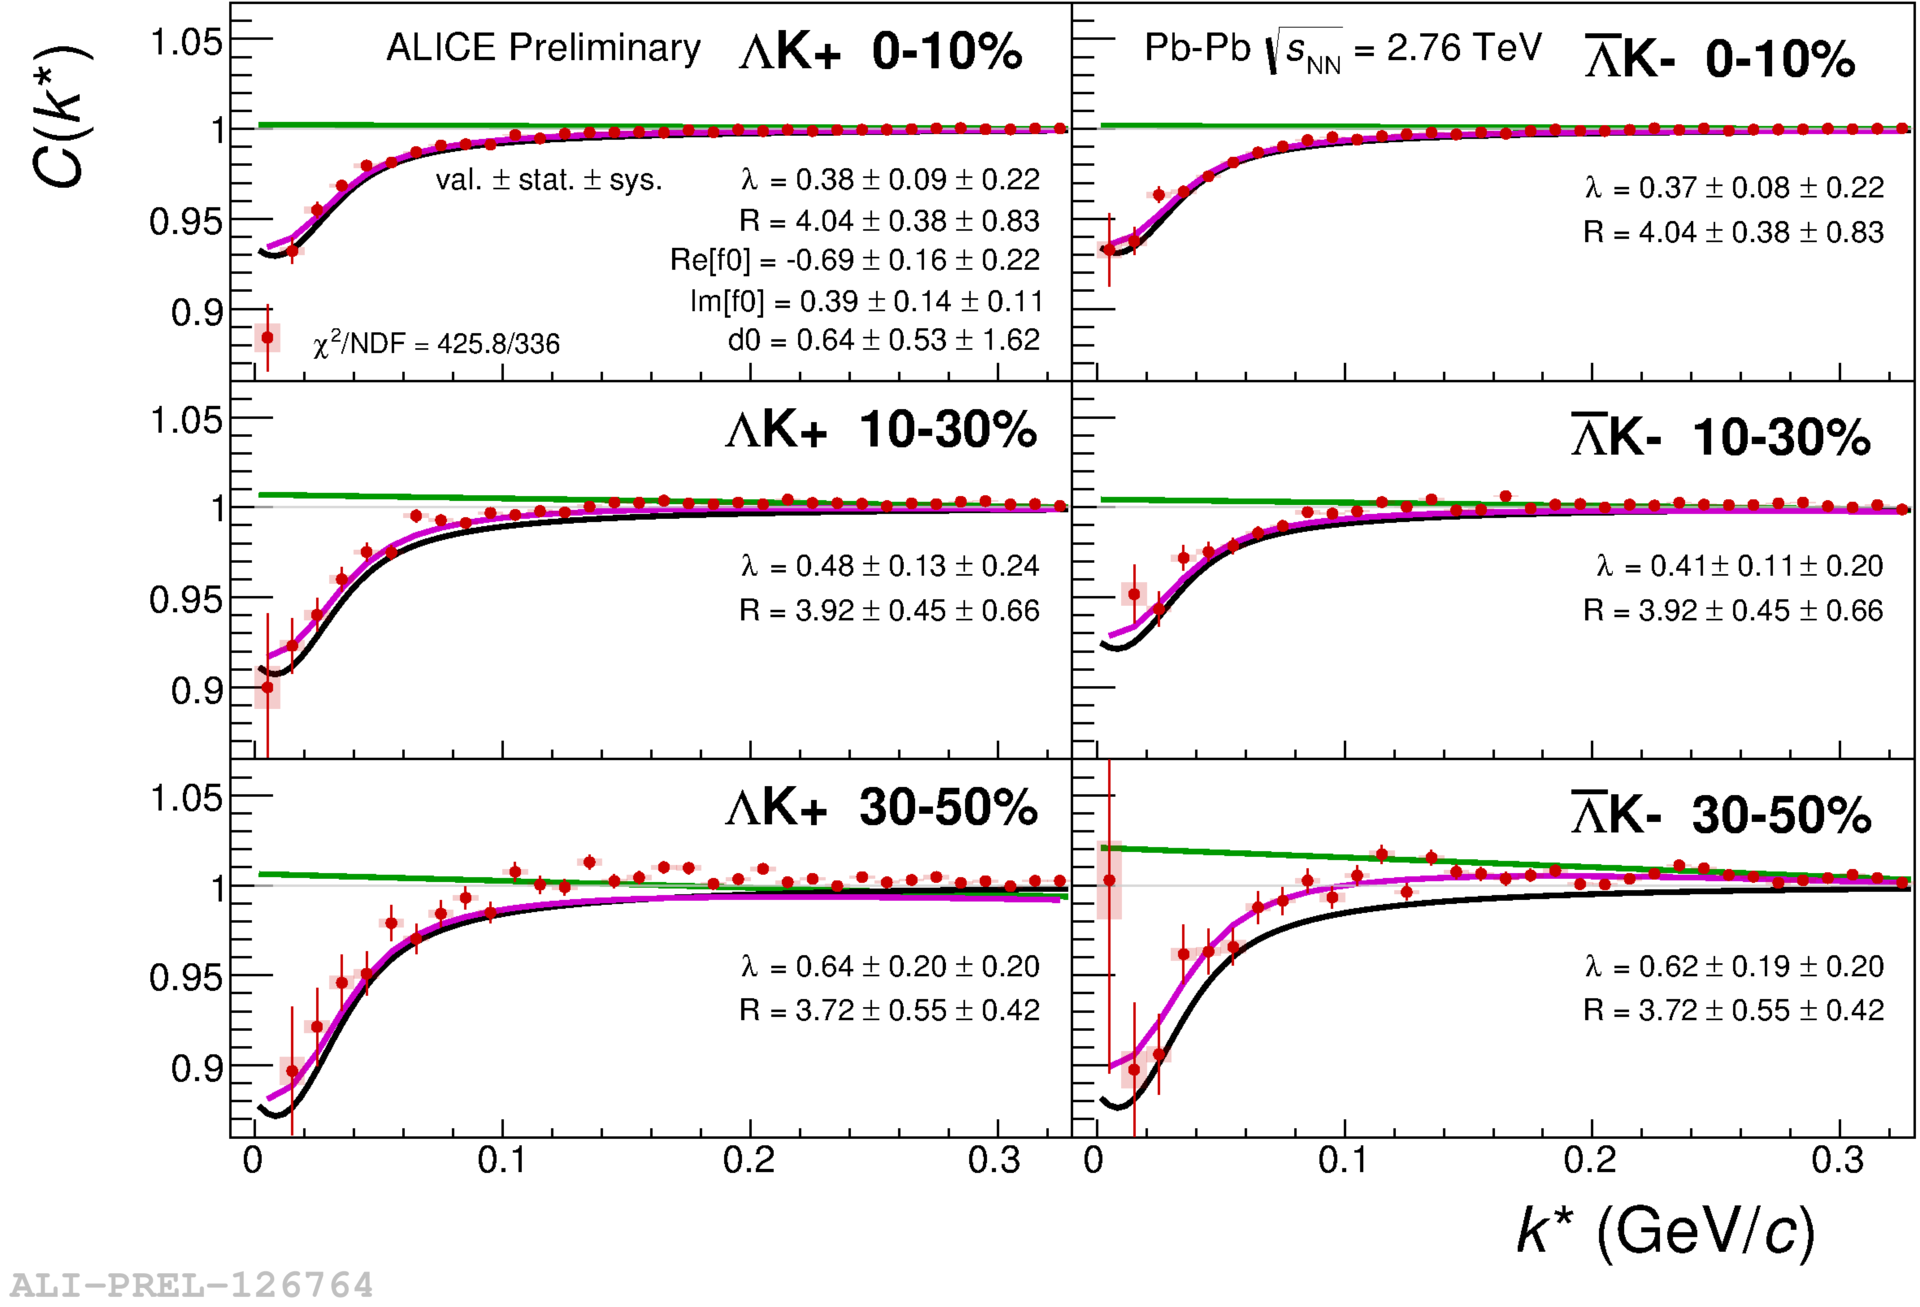
\includegraphics[width=\textwidth]{7_ResultsAndDiscussion/Figures/2017-Feb-04-canKStarCfwFitsLamKchPwConj_0010_1030_3050_MomResCrctn_NonFlatBgdCrctn.png}
  \caption[$\Lambda$K$^{+}$($\bar{\Lambda}$K$^{-}$) Fits]{Fits to the $\Lambda$K$^{+}$ (left) and $\bar{\Lambda}$K$^{-}$ (right) data for the centralities 0-10\% (top), 10-30\% (middle), and 30-50\% (bottom).
The lines represent the statistical errors, while the boxes represent the systematic errors.  
Each has unique $\lambda$ and normalization parameters.
The radii are shared amongst like centralities; the scattering parameters ($\mathbb{R}f_{0}$, $\mathbb{I}f_{0}$, $d_{0}$) are shared amongst all.
The black solid line represents the ``raw" fit, i.e. not corrected for momentum resolution effects nor non-flat background.  
The green line shows the fit to the non-flat background.
The purple points show the fit after momentum resolution and non-flat background corrections have been applied.
The initial values of the parameters is listed, as well as the final fit values with uncertainties.}
  \label{fig:LamKchPwConjFits}
\end{figure}

\begin{figure}[h]
  \centering
  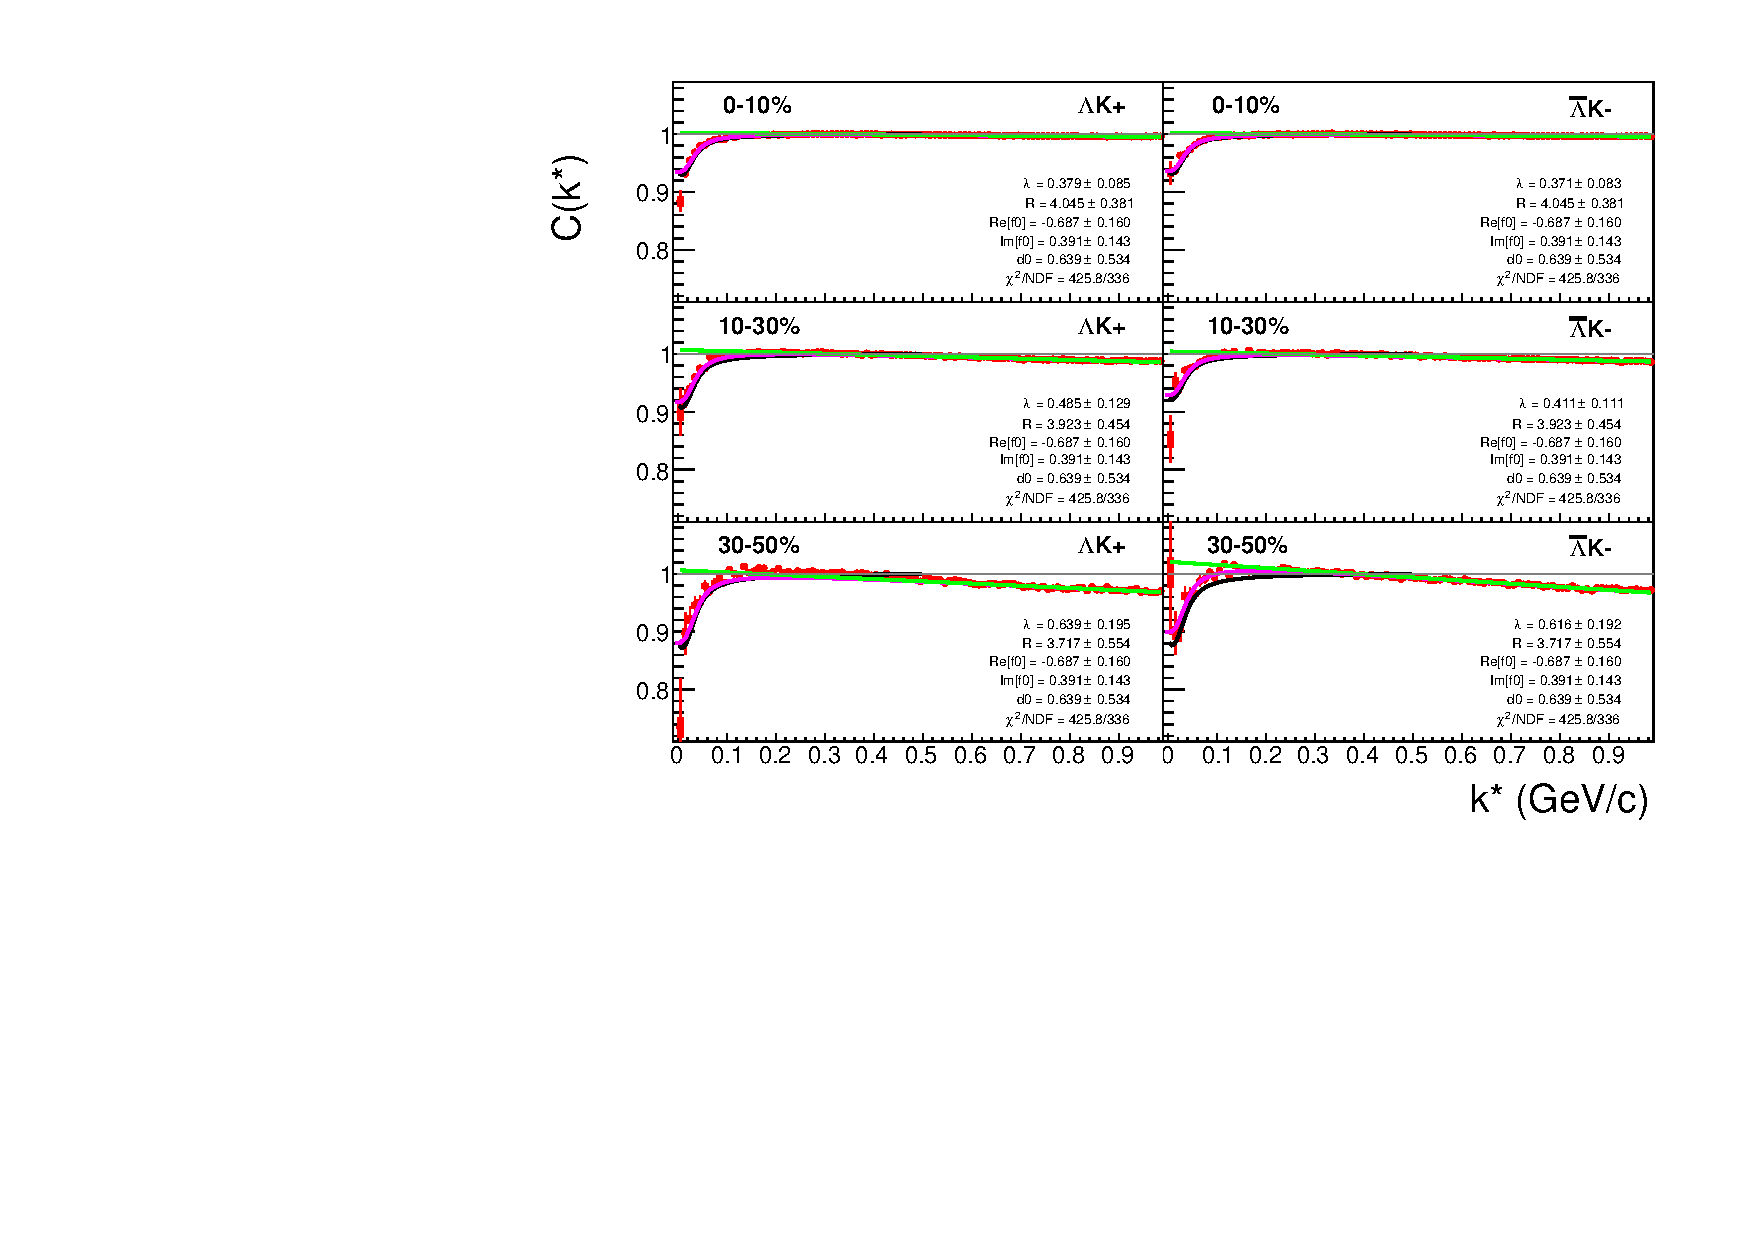
\includegraphics[width=\textwidth]{7_ResultsAndDiscussion/Figures/canKStarCfwFitsLamKchPwConj_0010_1030_3050UnZoomed_MomResCrctn_NonFlatBgdCrctn.pdf}
  \caption[$\Lambda$K$^{+}$($\bar{\Lambda}$K$^{-}$) Fits (Wide Range)]{Same as Fig. \ref{fig:LamKchPwConjFits}, but with a wider range of view.
Fits to the $\Lambda$K$^{+}$ (left) and $\bar{\Lambda}$K$^{-}$ (right) data for the centralities 0-10\% (top), 10-30\% (middle), and 30-50\% (bottom).
The lines represent the statistical errors, while the boxes represent the systematic errors.  
Each has unique $\lambda$ and normalization parameters.
The radii are shared amongst like centralities; the scattering parameters ($\mathbb{R}f_{0}$, $\mathbb{I}f_{0}$, $d_{0}$) are shared amongst all.
The black solid line represents the ``raw" fit, i.e. not corrected for momentum resolution effects nor non-flat background.  
The green line shows the fit to the non-flat background.
The purple points show the fit after momentum resolution and non-flat background corrections have been applied.
The initial values of the parameters is listed, as well as the final fit values with uncertainties.}
  \label{fig:LamKchPwConjFitsUnZoomed}
\end{figure}




\begin{figure}[h]
  \centering
  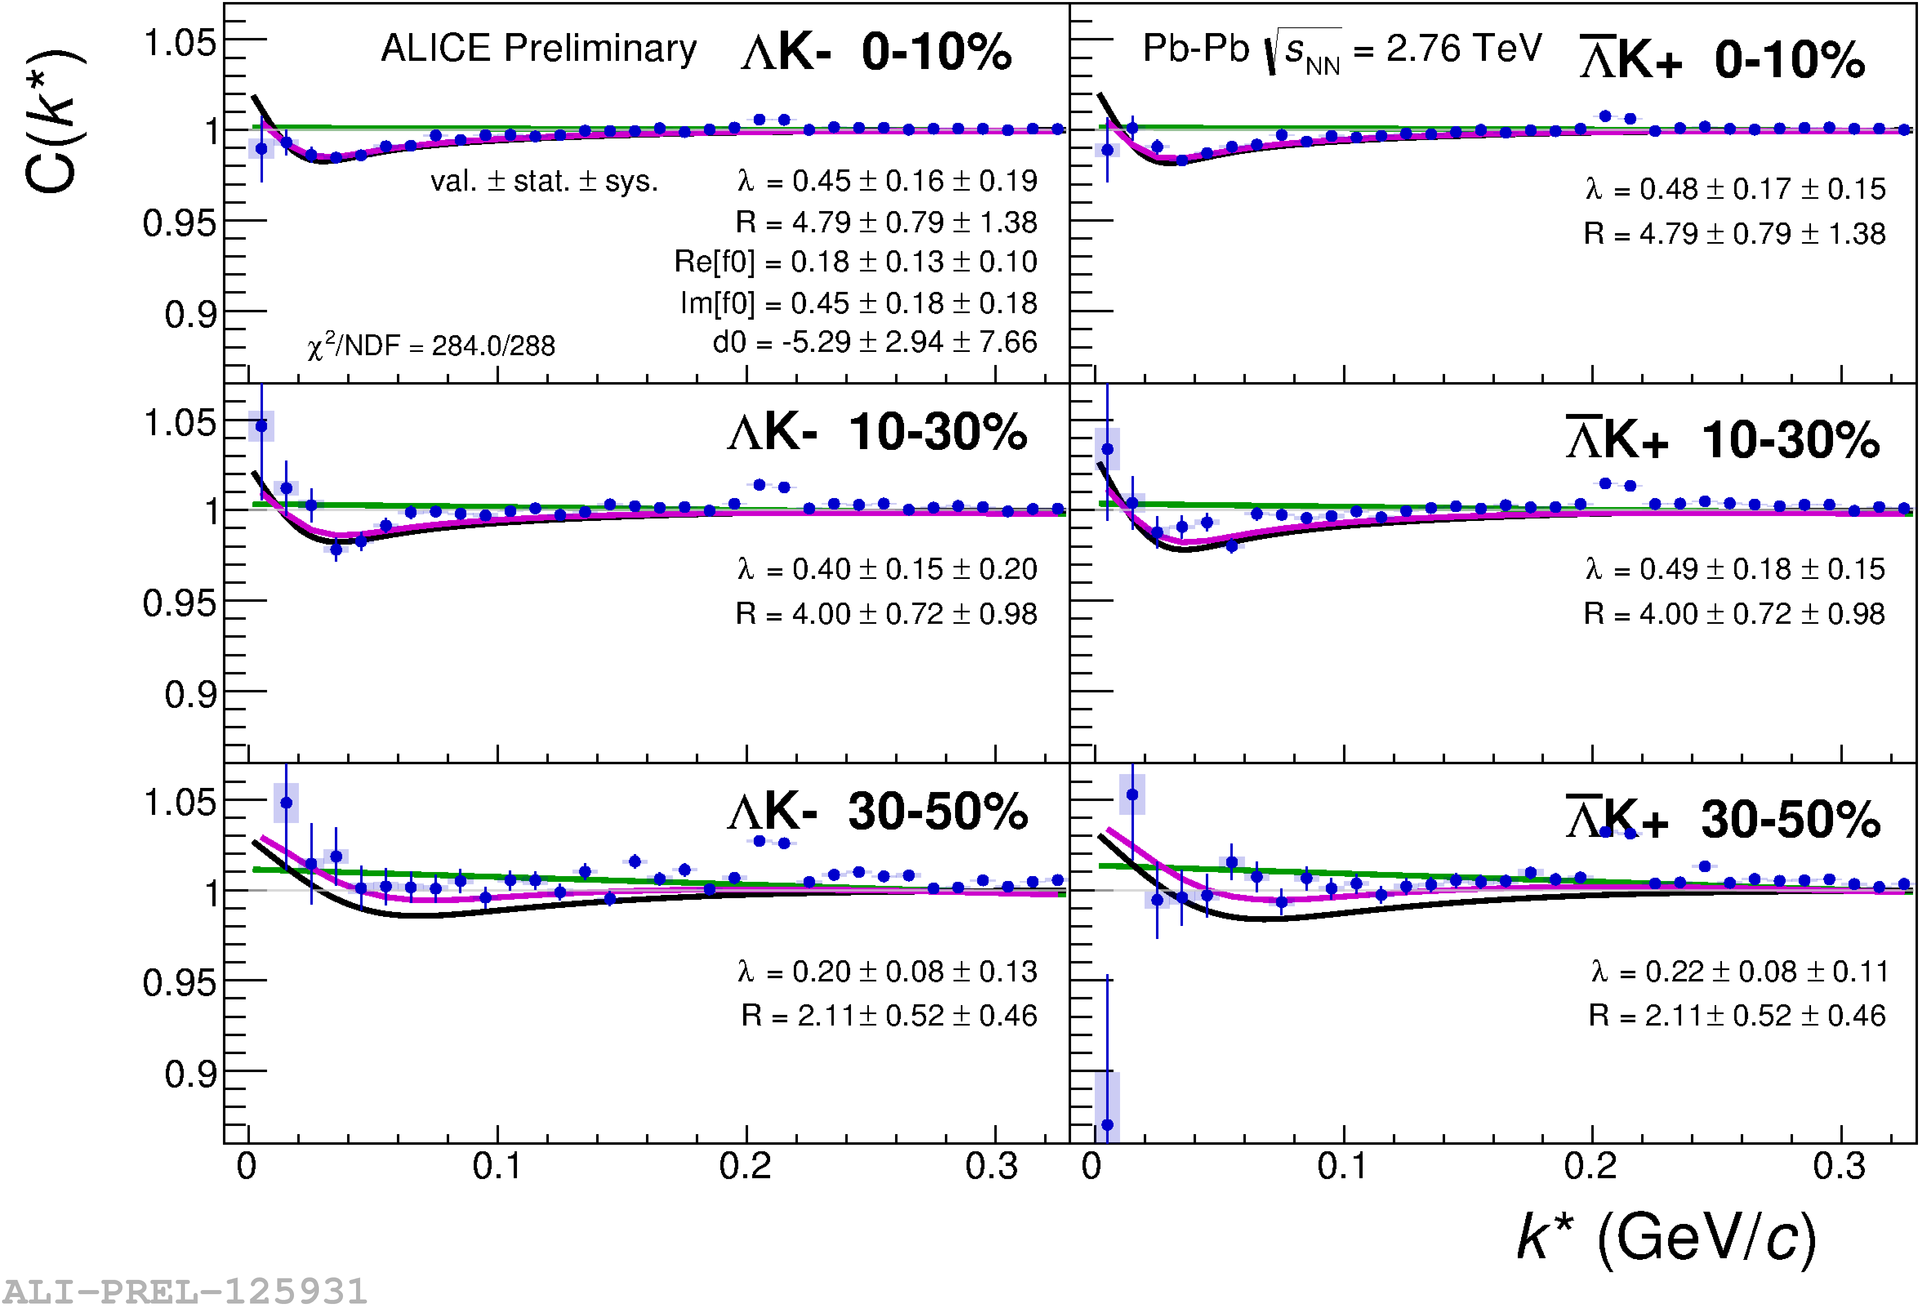
\includegraphics[width=\textwidth]{7_ResultsAndDiscussion/Figures/2017-Feb-03-canKStarCfwFitsLamKchMwConj_0010_1030_3050_MomResCrctn_NonFlatBgdCrctn.png}
  \caption[$\Lambda$K$^{-}$($\bar{\Lambda}$K$^{+}$) Fits]{Fits to the $\Lambda$K$^{-}$(left) with $\bar{\Lambda}$K$^{+}$ (right) data for the centralities 0-10\% (top), 10-30\% (middle), and 30-50\% (bottom).
The lines represent the statistical errors, while the boxes represent the systematic errors.  
Each has unique $\lambda$ and normalization parameters.
The radii are shared amongst like centralities; the scattering parameters ($\mathbb{R}f_{0}$, $\mathbb{I}f_{0}$, $d_{0}$) are shared amongst all.
The black solid line represents the ``raw" fit, i.e. not corrected for momentum resolution effects nor non-flat background.  
The green line shows the fit to the non-flat background.
The purple points show the fit after momentum resolution and non-flat background corrections have been applied.
The initial values of the parameters is listed, as well as the final fit values with uncertainties.}
  \label{fig:LamKchMwConjFits}
\end{figure}

\begin{figure}[h]
  \centering
  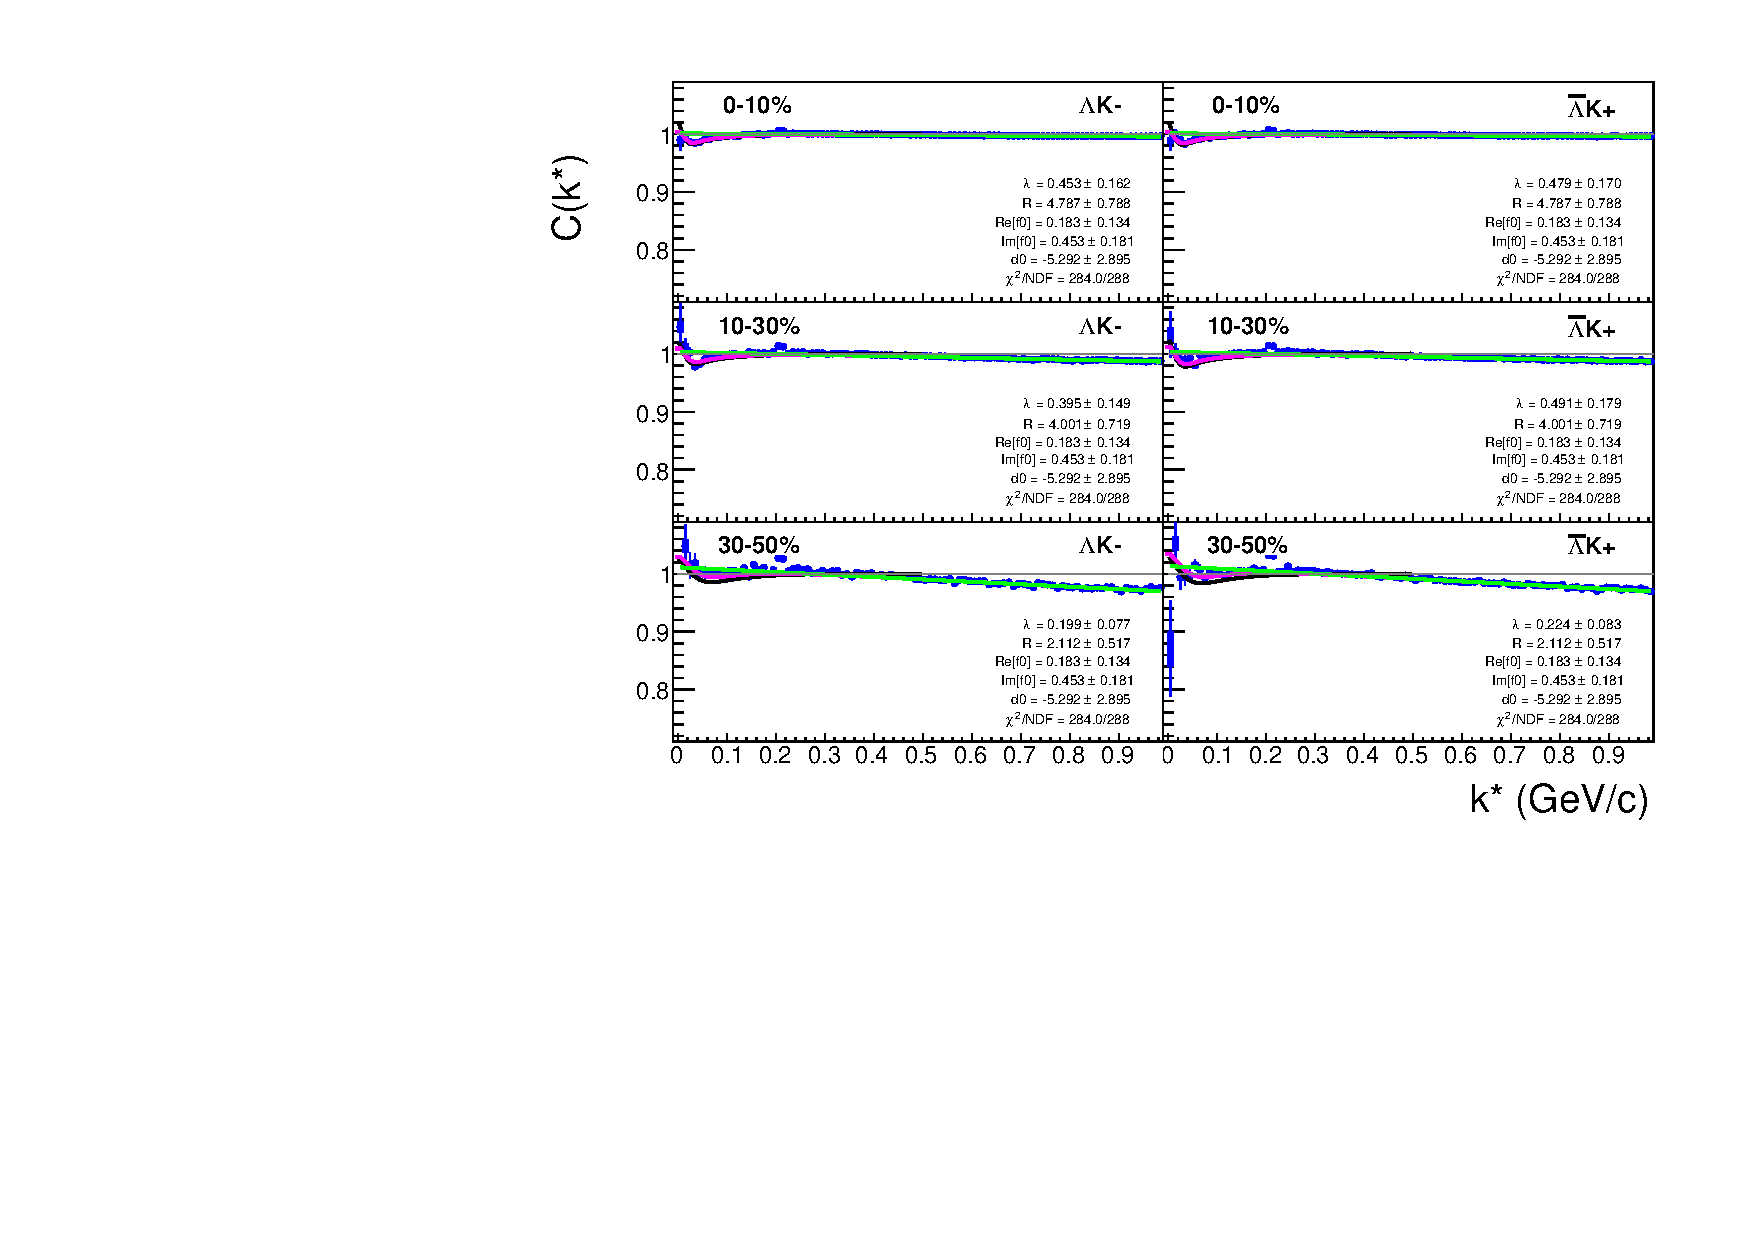
\includegraphics[width=\textwidth]{7_ResultsAndDiscussion/Figures/canKStarCfwFitsLamKchMwConj_0010_1030_3050UnZoomed_MomResCrctn_NonFlatBgdCrctn.pdf}
  \caption[$\Lambda$K$^{-}$($\bar{\Lambda}$K$^{+}$) Fits (Wide Range)]{Same as Fig. \ref{fig:LamKchMwConjFits}, but with a wider range of view.
Fits to the $\Lambda$K$^{-}$(left) with $\bar{\Lambda}$K$^{+}$ (right) data for the centralities 0-10\% (top), 10-30\% (middle), and 30-50\% (bottom).
The lines represent the statistical errors, while the boxes represent the systematic errors.  
Each has unique $\lambda$ and normalization parameters.
The radii are shared amongst like centralities; the scattering parameters ($\mathbb{R}f_{0}$, $\mathbb{I}f_{0}$, $d_{0}$) are shared amongst all.
The black solid line represents the ``raw" fit, i.e. not corrected for momentum resolution effects nor non-flat background.  
The green line shows the fit to the non-flat background.
The purple points show the fit after momentum resolution and non-flat background corrections have been applied.
The initial values of the parameters is listed, as well as the final fit values with uncertainties.}
  \label{fig:LamKchMwConjFitsUnZoomed}
\end{figure}




\pagestyle{empty}
\begin{landscape}


%%%%%%%%%%%%%%%%%%%%%%%%%%%%%%%%%%%%%%%%%%%%%%%%%%%%%%%%%%%%%%%%%%%%%%%%%%%%%%%%%%%%%%%%%%%%%%%%%%%%%%%%%%%%%%%%%%%%%%%%%%%
\begin{comment}
\begin{table}[htbp]
 \centering
 \resizebox{\paperwidth}{!}{
 \begin{tabular}{|c|c|c|c|c|c|c|}
  \multicolumn{7}{c}{Fit Results $\Lambda$($\bar{\Lambda}$)K$^{0}_{S}$} \\
  \hline
  \multirow{3}{*}{Pair Type} & \multirow{3}{*}{Centrality} & \multicolumn{5}{c|}{Fit Parameters} \\
  \cline{3-7}
   & & $\lambda$ & $R$ & $\mathbb{R}f_{0}$ & $\mathbb{I}f_{0}$ & $d_{0}$ \\
  \hline  
  \multirow{3}{*}{$\Lambda$K$^{0}_{S}$}  
   &  0-10\% & 0.654 $\pm$ 0.539 (stat.) $\pm$ 0.074 (sys.)  %Lambda
             & 3.863 $\pm$ 0.875 (stat.) $\pm$ 0.324 (sys.)  %Radius
             & \multirow{6}{*}{-0.116 $\pm$ 0.053 (stat.) $\pm$ 0.094 (sys.)}  %Ref0
             & \multirow{6}{*}{0.194 $\pm$ 0.109 (stat.) $\pm$ 0.056 (sys.)}  %Imf0
             & \multirow{6}{*}{3.627 $\pm$ 1.568 (stat.) $\pm$ 0.890 (sys.)} \\ %d0
             
   & 10-30\% & 0.312 $\pm$ 0.143 (stat.) $\pm$ 0.020 (sys.)  %Lambda
             & 2.000 $\pm$ 0.500 (stat.) $\pm$ 0.000 (sys.)  %Radius
             & & & \\
             
   & 30-50\% & 0.800 $\pm$ 0.400 (stat.) $\pm$ 0.124 (sys.)  %Lambda
             & 2.349 $\pm$ 0.561 (stat.) $\pm$ 0.230 (sys.)  %Radius
             & & & \\
  \cline{1-4}  
  \multirow{3}{*}{$\bar{\Lambda}$K$^{0}_{S}$}  
   &  0-10\% & 0.623 $\pm$ 0.526 (stat.) $\pm$ 0.058 (sys.)  %Lambda
             & 3.863 $\pm$ 0.875 (stat.) $\pm$ 0.324 (sys.)  %Radius
             & & & \\
             
   & 10-30\% & 0.326 $\pm$ 0.148 (stat.) $\pm$ 0.021 (sys.)  %Lambda
             & 2.000 $\pm$ 0.500 (stat.) $\pm$ 0.000 (sys.)  %Radius
             & & & \\
             
   & 30-50\% & 0.757 $\pm$ 0.140 (stat.) $\pm$ 0.093 (sys.)  %Lambda
             & 2.349 $\pm$ 0.561 (stat.) $\pm$ 0.230 (sys.)  %Radius
             & & & \\
  \hline
 \end{tabular}}
 \caption{Fit Results $\Lambda$($\bar{\Lambda}$)K$^{0}_{S}$. 
 Each pair is fit simultaneously with its conjugate (ie. $\Lambda$K$^{0}_{S}$ with $\bar{\Lambda}$K$^{0}_{S}$) across all centralities (0-10\%, 10-30\%, 30-50\%), for a total of 6 simultaneous analyses in the fit.
 Each analysis has a unique $\lambda$ and normalization parameter.
 The radii are shared between analyses of like centrality, as these should have similar source sizes.
 The scattering parameters ($\mathbb{R}f_{0}$, $\mathbb{I}f_{0}$, $d_{0}$) are shared amongst all.
 The fit is done on the data with only statistical error bars.
 The errors marked as ``stat." are those returned by MINUIT.
 The errors marked as ``sys." are those which result from my systematic analysis (as outlined in Section \ref{SystematicErrors}).}
 \label{tab:FitResultsLamK0}
\end{table}
\end{comment}
%%%%%%%%%%%%%%%%%%%%%%%%%%%%%%%%%%%%%%%%%%%%%%%%%%%%%%%%%%%%%%%%%%%%%%%%%%%%%%%%%%%%%%%%%%%%%%%%%%%%%%%%%%%%%%%%%%%%%%%%%%%


\begin{table}[htbp]
 \centering
 \resizebox{\paperwidth}{!}{
 \begin{tabular}{|c|c|c|c|c|c|c|}
  \multicolumn{7}{c}{Fit Results $\Lambda$($\bar{\Lambda}$)K$^{0}_{S}$} \\
  \hline
  \multirow{3}{*}{Pair Type} & \multirow{3}{*}{Centrality} & \multicolumn{5}{c|}{Fit Parameters} \\
  \cline{3-7}
   & & $\lambda$ & $R$ & $\mathbb{R}f_{0}$ & $\mathbb{I}f_{0}$ & $d_{0}$ \\
  \hline  
  \multirow{3}{*}{$\Lambda$K$^{0}_{S}$}  
   &  0-10\% & \multirow{6}{*}{0.400 $\pm$ 0.187 (stat.) $\pm$ 0.116 (sys.)}  %Lambda
             & 3.024 $\pm$ 0.541 (stat.) $\pm$ 0.329 (sys.)  %Radius
             & \multirow{6}{*}{-0.157 $\pm$ 0.031 (stat.) $\pm$ 0.043 (sys.)}  %Ref0
             & \multirow{6}{*}{0.176 $\pm$ 0.077 (stat.) $\pm$ 0.059 (sys.)}  %Imf0
             & \multirow{6}{*}{3.566 $\pm$ 0.947 (stat.) $\pm$ 2.836 (sys.)} \\ %d0
             
   & 10-30\% & 
             & 2.270 $\pm$ 0.413 (stat.) $\pm$ 0.324 (sys.)  %Radius
             & & & \\
             
   & 30-50\% & 
             & 1.669 $\pm$ 0.307 (stat.) $\pm$ 0.280 (sys.)  %Radius
             & & & \\
  \cline{1-2}
  \cline{4-4}
  \multirow{3}{*}{$\bar{\Lambda}$K$^{0}_{S}$}  
   &  0-10\% & 
             & 3.024 $\pm$ 0.541 (stat.) $\pm$ 0.329 (sys.)  %Radius
             & & & \\
             
   & 10-30\% & 
             & 2.270 $\pm$ 0.413 (stat.) $\pm$ 0.324 (sys.)  %Radius
             & & & \\
             
   & 30-50\% & 
             & 1.669 $\pm$ 0.307 (stat.) $\pm$ 0.280 (sys.)  %Radius
             & & & \\
  \hline
 \end{tabular}}
 \caption{Fit Results $\Lambda$($\bar{\Lambda}$)K$^{0}_{S}$. 
 Each pair is fit simultaneously with its conjugate (ie. $\Lambda$K$^{0}_{S}$ with $\bar{\Lambda}$K$^{0}_{S}$) across all centralities (0-10\%, 10-30\%, 30-50\%), for a total of 6 simultaneous analyses in the fit.
 Each analysis has a unique $\lambda$ and normalization parameter.
 The radii are shared between analyses of like centrality, as these should have similar source sizes.
 The scattering parameters ($\mathbb{R}f_{0}$, $\mathbb{I}f_{0}$, $d_{0}$) are shared amongst all.
 The fit is done on the data with only statistical error bars.
 The errors marked as ``stat." are those returned by MINUIT.
 The errors marked as ``sys." are those which result from my systematic analysis (as outlined in Section \ref{SystematicErrors}).}
 \label{tab:FitResultsLamK0}
\end{table}



%\end{landscape}
%\pagestyle{plain}

%\pagestyle{empty}
%\begin{landscape}

\begin{table}[htbp]
 \centering
 \resizebox{\paperwidth}{!}{
 \begin{tabular}{|c|c|c|c|c|c|c|}
  \multicolumn{7}{c}{Fit Results $\Lambda$($\bar{\Lambda}$)K$^{\pm}$} \\
  \hline
  \multirow{3}{*}{Pair Type} & \multirow{3}{*}{Centrality} & \multicolumn{5}{c|}{Fit Parameters} \\
  \cline{3-7}
   & & $\lambda$ & $R$ & $\mathbb{R}f_{0}$ & $\mathbb{I}f_{0}$ & $d_{0}$ \\
  \hline  
  \multirow{3}{*}{$\Lambda$K$^{+}$}  
   &  0-10\% & 0.379 $\pm$ 0.085 (stat.) $\pm$ 0.220 (sys.)  %Lambda
             & 4.045 $\pm$ 0.381 (stat.) $\pm$ 0.830 (sys.)  %Radius
             & \multirow{6}{*}{-0.687 $\pm$ 0.160 (stat.) $\pm$ 0.223 (sys.)}  %Ref0
             & \multirow{6}{*}{0.391 $\pm$ 0.143 (stat.) $\pm$ 0.111 (sys.)}  %Imf0
             & \multirow{6}{*}{0.639 $\pm$ 0.534 (stat.) $\pm$ 1.621 (sys.)} \\ %d0
             
   & 10-30\% & 0.485 $\pm$ 0.129 (stat.) $\pm$ 0.241 (sys.)  %Lambda
             & 3.923 $\pm$ 0.454 (stat.) $\pm$ 0.663 (sys.)  %Radius
             & & & \\
             
   & 30-50\% & 0.639 $\pm$ 0.195 (stat.) $\pm$ 0.204 (sys.)  %Lambda
             & 3.717 $\pm$ 0.554 (stat.) $\pm$ 0.420 (sys.)  %Radius
             & & & \\
  \cline{1-4}  
  \multirow{3}{*}{$\bar{\Lambda}$K$^{-}$}  
   &  0-10\% & 0.371 $\pm$ 0.083 (stat.) $\pm$ 0.217 (sys.)  %Lambda
             & 4.045 $\pm$ 0.381 (stat.) $\pm$ 0.830 (sys.)  %Radius
             & & & \\
             
   & 10-30\% & 0.411 $\pm$ 0.111 (stat.) $\pm$ 0.201 (sys.)  %Lambda
             & 3.923 $\pm$ 0.454 (stat.) $\pm$ 0.663 (sys.)  %Radius
             & & & \\
             
   & 30-50\% & 0.616 $\pm$ 0.192 (stat.) $\pm$ 0.203 (sys.)  %Lambda
             & 3.717 $\pm$ 0.554 (stat.) $\pm$ 0.420 (sys.)  %Radius
             & & & \\
  \hline
  \hline  
  \multirow{3}{*}{$\Lambda$K$^{-}$}  
   &  0-10\% & 0.453 $\pm$ 0.162 (stat.) $\pm$ 0.186 (sys.)  %Lambda
             & 4.787 $\pm$ 0.788 (stat.) $\pm$ 1.375 (sys.)  %Radius
             & \multirow{6}{*}{0.183 $\pm$ 0.134 (stat.) $\pm$ 0.095 (sys.)}  %Ref0
             & \multirow{6}{*}{0.453 $\pm$ 0.181 (stat.) $\pm$ 0.184 (sys.)}  %Imf0
             & \multirow{6}{*}{-5.292 $\pm$ 2.895 (stat.) $\pm$ 7.658 (sys.)} \\ %d0
             
   & 10-30\% & 0.395 $\pm$ 0.149 (stat.) $\pm$ 0.198 (sys.)  %Lambda
             & 4.001 $\pm$ 0.719 (stat.) $\pm$ 0.978 (sys.)  %Radius
             & & & \\
             
   & 30-50\% & 0.199 $\pm$ 0.077 (stat.) $\pm$ 0.132 (sys.)  %Lambda
             & 2.112 $\pm$ 0.517 (stat.) $\pm$ 0.457 (sys.)  %Radius
             & & & \\
  \cline{1-4}  
  \multirow{3}{*}{$\bar{\Lambda}$K$^{+}$}  
   &  0-10\% & 0.479 $\pm$ 0.170 (stat.) $\pm$ 0.152 (sys.)  %Lambda
             & 4.787 $\pm$ 0.788 (stat.) $\pm$ 1.375 (sys.)  %Radius
             & & & \\
             
   & 10-30\% & 0.491 $\pm$ 0.179 (stat.) $\pm$ 0.148 (sys.)  %Lambda
             & 4.001 $\pm$ 0.719 (stat.) $\pm$ 0.978 (sys.)  %Radius
             & & & \\
             
   & 30-50\% & 0.224 $\pm$ 0.083 (stat.) $\pm$ 0.106 (sys.)  %Lambda
             & 2.112 $\pm$ 0.517 (stat.) $\pm$ 0.457 (sys.)  %Radius
             & & & \\
  \hline
 \end{tabular}}
 \caption{Fit Results $\Lambda$($\bar{\Lambda}$)K$^{\pm}$
 Each pair is fit simultaneously with its conjugate (ie. $\Lambda$K$^{+}$ with $\bar{\Lambda}$K$^{-}$ and $\Lambda$K$^{-}$ with $\bar{\Lambda}$K$^{+}$) across all centralities (0-10\%, 10-30\%, 30-50\%), for a total of 6 simultaneous analyses in the fit.
 Each analysis has a unique $\lambda$ and normalization parameter.
 The radii are shared between analyses of like centrality, as these should have similar source sizes.
 The scattering parameters ($\mathbb{R}f_{0}$, $\mathbb{I}f_{0}$, $d_{0}$) are shared amongst all.
 The fit is done on the data with only statistical error bars.
 The errors marked as ``stat." are those returned by MINUIT.
 The errors marked as ``sys." are those which result from my systematic analysis (as outlined in Section \ref{SystematicErrors}).}
 \label{tab:FitResultsLamKch}
\end{table}

%%%%%%%%%%%%%%%%%%%%%%%%%%%%%%%%%%%%%%%%%%%%%%%%%%%%%%%%%%%%%%%%%%%%%%%%%%%%%%%%%%%%%%%%%%%%%
\begin{comment}
\begin{table}[htbp]
 \centering
 \resizebox{\paperwidth}{!}{
 \begin{tabular}{|c|c|c|c|c|c|c|}
  \multicolumn{7}{c}{Fit Results $\Lambda$($\bar{\Lambda}$)K$^{0}_{S}$} \\
  \hline
  \multirow{3}{*}{Pair Type} & \multirow{3}{*}{Centrality} & \multicolumn{5}{c|}{Fit Parameters} \\
  \cline{3-7}
   & & $\lambda$ & $R$ & $\mathbb{R}f_{0}$ & $\mathbb{I}f_{0}$ & $d_{0}$ \\
  \hline  
  \multirow{3}{*}{$\Lambda$K$^{0}_{S}$}  
   &  0-10\% & 0.654 $\pm$ 0.539 (stat.) $\pm$ 0.074 (sys.)  %Lambda
             & 3.863 $\pm$ 0.875 (stat.) $\pm$ 0.324 (sys.)  %Radius
             & \multirow{6}{*}{-0.116 $\pm$ 0.053 (stat.) $\pm$ 0.094 (sys.)}  %Ref0
             & \multirow{6}{*}{0.194 $\pm$ 0.109 (stat.) $\pm$ 0.056 (sys.)}  %Imf0
             & \multirow{6}{*}{3.627 $\pm$ 1.568 (stat.) $\pm$ 0.890 (sys.)} \\ %d0
             
   & 10-30\% & 0.312 $\pm$ 0.143 (stat.) $\pm$ 0.020 (sys.)  %Lambda
             & 2.000 $\pm$ 0.500 (stat.) $\pm$ 0.000 (sys.)  %Radius
             & & & \\
             
   & 30-50\% & 0.800 $\pm$ 0.400 (stat.) $\pm$ 0.124 (sys.)  %Lambda
             & 2.349 $\pm$ 0.561 (stat.) $\pm$ 0.230 (sys.)  %Radius
             & & & \\
  \cline{1-4}  
  \multirow{3}{*}{$\bar{\Lambda}$K$^{0}_{S}$}  
   &  0-10\% & 0.623 $\pm$ 0.526 (stat.) $\pm$ 0.058 (sys.)  %Lambda
             & 3.863 $\pm$ 0.875 (stat.) $\pm$ 0.324 (sys.)  %Radius
             & & & \\
             
   & 10-30\% & 0.326 $\pm$ 0.148 (stat.) $\pm$ 0.021 (sys.)  %Lambda
             & 2.000 $\pm$ 0.500 (stat.) $\pm$ 0.000 (sys.)  %Radius
             & & & \\
             
   & 30-50\% & 0.757 $\pm$ 0.140 (stat.) $\pm$ 0.093 (sys.)  %Lambda
             & 2.349 $\pm$ 0.561 (stat.) $\pm$ 0.230 (sys.)  %Radius
             & & & \\
  \hline
  \hline  
  \hline
  \multirow{3}{*}{$\Lambda$K$^{+}$}  
   &  0-10\% & 0.379 $\pm$ 0.088 (stat.) $\pm$ 0.205 (sys.)  %Lambda
             & 4.045 $\pm$ 0.202 (stat.) $\pm$ 1.076 (sys.)  %Radius
             & \multirow{6}{*}{-0.687 $\pm$ 0.151 (stat.) $\pm$ 0.107 (sys.)}  %Ref0
             & \multirow{6}{*}{0.391 $\pm$ 0.107 (stat.) $\pm$ 0.212 (sys.)}  %Imf0
             & \multirow{6}{*}{0.639 $\pm$ 0.507 (stat.) $\pm$ 2.378 (sys.)} \\ %d0
             
   & 10-30\% & 0.485 $\pm$ 0.098 (stat.) $\pm$ 0.157 (sys.)  %Lambda
             & 3.923 $\pm$ 0.318 (stat.) $\pm$ 0.926 (sys.)  %Radius
             & & & \\
             
   & 30-50\% & 0.639 $\pm$ 0.157 (stat.) $\pm$ 0.092 (sys.)  %Lambda
             & 3.716 $\pm$ 0.411 (stat.) $\pm$ 0.460 (sys.)  %Radius
             & & & \\
  \cline{1-4}  
  \multirow{3}{*}{$\bar{\Lambda}$K$^{-}$}  
   &  0-10\% & 0.371 $\pm$ 0.086 (stat.) $\pm$ 0.193 (sys.)  %Lambda
             & 4.045 $\pm$ 0.202 (stat.) $\pm$ 1.076 (sys.)  %Radius
             & & & \\
             
   & 10-30\% & 0.411 $\pm$ 0.085 (stat.) $\pm$ 0.116 (sys.)  %Lambda
             & 3.923 $\pm$ 0.318 (stat.) $\pm$ 0.926 (sys.)  %Radius
             & & & \\
             
   & 30-50\% & 0.616 $\pm$ 0.154 (stat.) $\pm$ 0.071 (sys.)  %Lambda
             & 3.716 $\pm$ 0.411 (stat.) $\pm$ 0.460 (sys.)  %Radius
             & & & \\
  \hline
  \hline  
  \multirow{3}{*}{$\Lambda$K$^{-}$}  
   &  0-10\% & 0.453 $\pm$ 0.172 (stat.) $\pm$ 0.080 (sys.)  %Lambda
             & 4.787 $\pm$ 0.795 (stat.) $\pm$ 0.270 (sys.)  %Radius
             & \multirow{6}{*}{0.183 $\pm$ 0.130 (stat.) $\pm$ 0.074 (sys.)}  %Ref0
             & \multirow{6}{*}{0.453 $\pm$ 0.183 (stat.) $\pm$ 0.162 (sys.)}  %Imf0
             & \multirow{6}{*}{-5.292 $\pm$ 2.935 (stat.) $\pm$ 3.748 (sys.)} \\ %d0
             
   & 10-30\% & 0.395 $\pm$ 0.154 (stat.) $\pm$ 0.052 (sys.)  %Lambda
             & 4.001 $\pm$ 0.716 (stat.) $\pm$ 0.215 (sys.)  %Radius
             & & & \\
             
   & 30-50\% & 0.199 $\pm$ 0.079 (stat.) $\pm$ 0.031 (sys.)  %Lambda
             & 2.112 $\pm$ 0.558 (stat.) $\pm$ 0.176 (sys.)  %Radius
             & & & \\
  \cline{1-4}  
  \multirow{3}{*}{$\bar{\Lambda}$K$^{+}$}  
   &  0-10\% & 0.479 $\pm$ 0.180 (stat.) $\pm$ 0.082 (sys.)  %Lambda
             & 4.787 $\pm$ 0.180 (stat.) $\pm$ 0.270 (sys.)  %Radius
             & & & \\
             
   & 10-30\% & 0.491 $\pm$ 0.185 (stat.) $\pm$ 0.061 (sys.)  %Lambda
             & 4.001 $\pm$ 0.716 (stat.) $\pm$ 0.215 (sys.)  %Radius
             & & & \\
             
   & 30-50\% & 0.224 $\pm$ 0.085 (stat.) $\pm$ 0.029 (sys.)  %Lambda
             & 2.112 $\pm$ 0.558 (stat.) $\pm$ 0.176 (sys.)  %Radius
             & & & \\
  \hline  
 \end{tabular}}
 \caption{Fit Results $\Lambda$($\bar{\Lambda}$)K$^{0}_{S}$}
 \label{tab:FitResultsAll}
\end{table}
\end{comment}
%%%%%%%%%%%%%%%%%%%%%%%%%%%%%%%%%%%%%%%%%%%%%%%%%%%%%%%%%%%%%%%%%%%%%%%%%%%%%%%%%%%%%%%%%%%%%
%%%%%%%%%%%%%%%%%% QM 17 Stuff %%%%%%%%%%%%%%%%%%%%%%%%%%%%%%%%%%%%%%%%%%%%%%%%%%%%%%%%%%%%%%

\clearpage
\begin{table}[htbp]
 \centering
 \resizebox{\paperwidth}{!}{
 \begin{tabular}{|c|c|c|c|c|}
  \multicolumn{2}{c}{} & \multicolumn{3}{c}{\textbf{\large Fit Parameters} (\large \textbf{value $\pm$ statistical error $\pm$ systematic error)}} \\
  \hline
  \textbf{\large Pair Type} & \textbf{\large Centrality} & \multicolumn{3}{c|}{\textbf{\large R}} \\
  \cline{1-5}
  \multirow{5}{*}{\large \textbf{$\Lambda$K$^{+}$ \& $\bar{\Lambda}$K$^{-}$}}
  &  \textbf{0-10\%} & \multicolumn{3}{c|}{\textbf{4.04 $\pm$ 0.38 $\pm$ 0.83}} \\  %Radius
  & \textbf{10-30\%} & \multicolumn{3}{c|}{\textbf{3.92 $\pm$ 0.45 $\pm$ 0.66}} \\  %Radius
  & \textbf{30-50\%} & \multicolumn{3}{c|}{\textbf{3.72 $\pm$ 0.55 $\pm$ 0.42}} \\  %Radius
  \cline{2-5}
  & & \large $\mathbf{\Re f_{0}}$ & \large $\mathbf{\Im f_{0}}$ & \large $\mathbf{d_{0}}$ \\
  \cline{3-5}  
  & & \textbf{-0.69 $\pm$ 0.16 $\pm$ 0.22} & \textbf{0.39 $\pm$ 0.14 $\pm$ 0.11} & \textbf{0.64 $\pm$ 0.53 $\pm$ 1.62} \\
  
  \hline
  \hline
  
  \multirow{5}{*}{\large \textbf{$\Lambda$K$^{-}$ \& $\bar{\Lambda}$K$^{+}$}} 
  &  \textbf{0-10\%} & \multicolumn{3}{c|}{\textbf{4.79 $\pm$ 0.79 $\pm$ 1.38}} \\  %Radius
  & \textbf{10-30\%} & \multicolumn{3}{c|}{\textbf{4.00 $\pm$ 0.72 $\pm$ 0.98}} \\  %Radius
  & \textbf{30-50\%} & \multicolumn{3}{c|}{\textbf{2.11 $\pm$ 0.52 $\pm$ 0.46}} \\  %Radius
  \cline{2-5}
  & & \large $\mathbf{\Re f_{0}}$ & \large $\mathbf{\Im f_{0}}$ & \large $\mathbf{d_{0}}$ \\
  \cline{3-5}     
  & & \textbf{0.18 $\pm$ 0.13 $\pm$ 0.10} & \textbf{0.45 $\pm$ 0.18 $\pm$ 0.18} & \textbf{-5.29 $\pm$ 2.94 $\pm$ 7.66} \\
   
  \hline
  \hline  
  
  \multirow{5}{*}{\large \textbf{$\Lambda$K$^{0}_{S}$ \& $\bar{\Lambda}$K$^{0}_{S}$}}  
   &  \textbf{0-10\%} & \multicolumn{3}{c|}{\textbf{3.02 $\pm$ 0.54 $\pm$ 0.33}} \\  %Radius
   & \textbf{10-30\%} & \multicolumn{3}{c|}{\textbf{2.27 $\pm$ 0.41 $\pm$ 0.32}} \\  %Radius
   & \textbf{30-50\%} & \multicolumn{3}{c|}{\textbf{1.67 $\pm$ 0.30 $\pm$ 0.28}} \\  %Radius
   \cline{2-5}   
   & & \large $\mathbf{\Re f_{0}}$ & \large $\mathbf{\Im f_{0}}$ & \large $\mathbf{d_{0}}$ \\
   \cline{3-5} 
   & & \textbf{-0.16 $\pm$ 0.03 $\pm$ 0.04} & \textbf{0.18 $\pm$ 0.08 $\pm$ 0.06} & \textbf{3.57 $\pm$ 0.95 $\pm$ 2.84} \\
  \hline
 \end{tabular}}
 \label{tab:FitResultsLamKchandLamK0QM2}
\end{table}

\end{landscape}
\pagestyle{plain}

Figure \ref{fig:mTScalingOfRadii} shows extracted $R_{\mathrm{inv}}$ parameters as a function of tranverse mass ($m_{\mathrm{T}}$) for various pair systems over several centralities.  The published ALICE data \cite{Adam:2015vja} is shown with transparent, open symbols.  The new $\Lambda$K results are shown with opaque, filled symbols.  The radii shown an increasing size with increasing centrality, as is expected from the simple geometric picture of the collisions.  The radii decrease in size with increasing $m_{\mathrm{T}}$, and we see an approximate scaling of the radii with transverse mass, as is expected in the presence of collective flow in the system.

\begin{figure}[h]
  \centering
  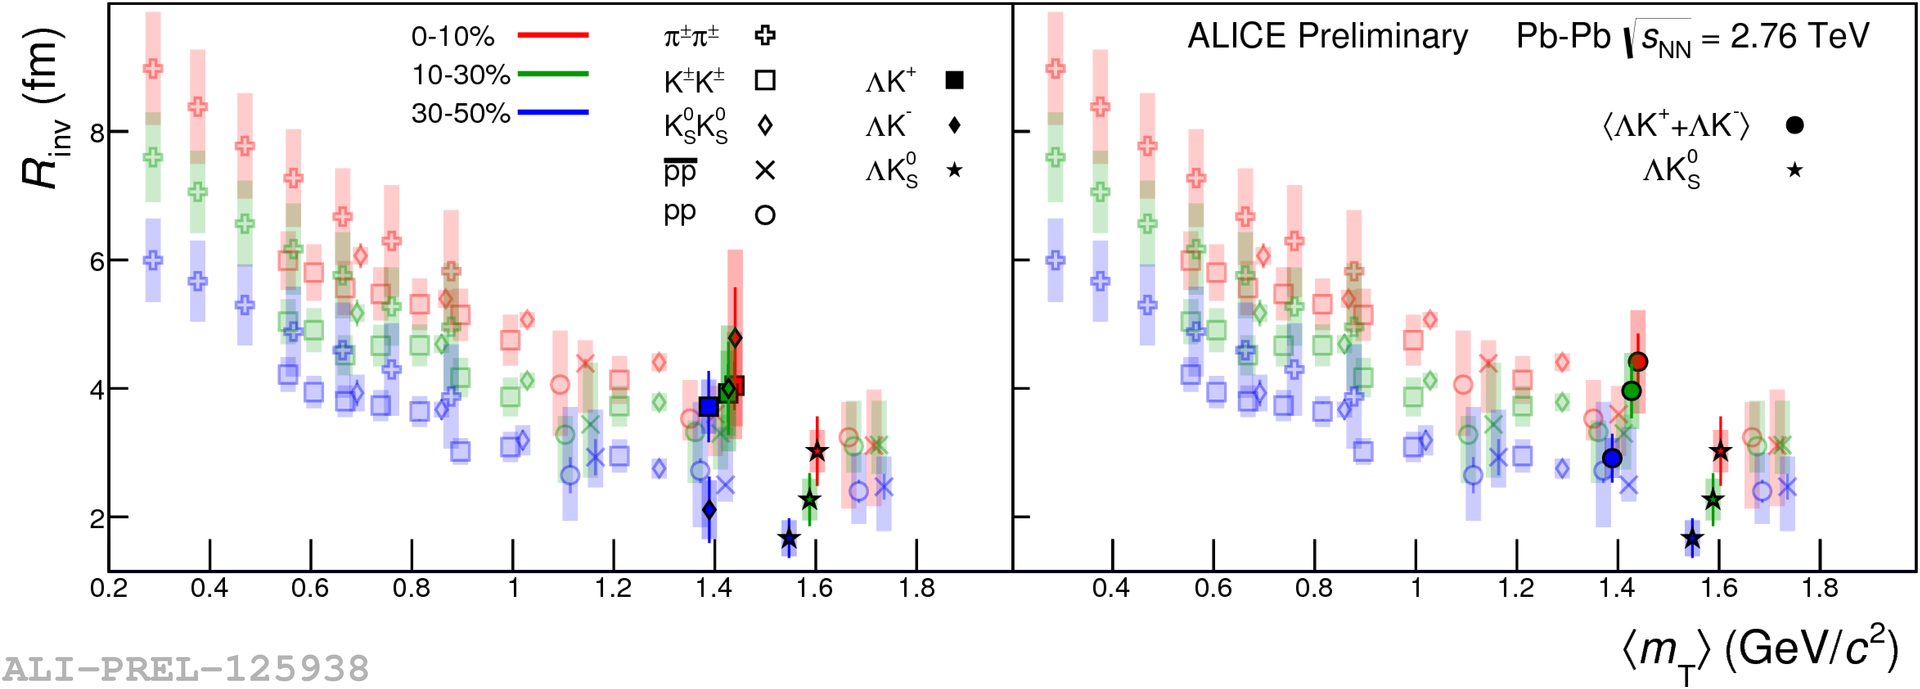
\includegraphics[width=\textwidth]{7_ResultsAndDiscussion/Figures/2017-Feb-03-mTscalingQMv2_MinvCalc_OutlinedPoints_OthersTransparent.png}
  \caption[$m_{\mathrm{T}}$ Scaling of Radii]{Extracted fit $R_{\mathrm{inv}}$ parameters as a function of pair transverse mass ($m_{\mathrm{T}}$) for various pair systems over several centralities. The ALICE published data \cite{Adam:2015vja} is shown with transparent, open symbols.  The new $\Lambda$K results are shown with opaque, filled symbols.  In the left, the $\Lambda$K$^{+}$ (with it's conjugate pair) results are shown separately from the $\Lambda$K$^{-}$ (with it's conjugate pair) results.  In the right, all $\Lambda$K$^{\pm}$ results are averaged.}
  \label{fig:mTScalingOfRadii}
\end{figure}

\end{document}